\chapter{Improved predictions for \decay{\Lb}{\Lz\mumu} observables.}
\label{app:newpredictions}

  The publication of the results included in this thesis triggered interest in the
  theory community, which produced improved lattice calculations and predictions~\cite{Detmold:2016pkz}.
  This section reports the measured quantities with the new predictions overlaid
  as reported in Ref.~\cite{Detmold:2016pkz}.
  
  
  \begin{table}[!h]
   \centering
 \begin{tabular}{c|cccc}
                                                                & \hspace{1ex}  & { \bf Prediction}            & \hspace{1ex}   & { \bf Measurement}              \\
 \hline
 $\langle \mathrm{d}\mathcal{B}/\mathrm{d} q^2\rangle_{[15,\,20]}$             && $0.756 \pm 0.070$    && $1.20\pm0.27$  \\
 $\langle F_L \rangle_{[15,\,20]} $                                         && $0.409 \pm 0.013$    && $0.61^{+\,0.11}_{-\,0.14}$   \\
 $\langle A_{\rm FB}^\ell \rangle_{[15,\,20]} $                             && $-0.350 \pm 0.013$      && $-0.05\pm0.09$    \\
 $\langle A_{\rm FB}^\Lambda \rangle_{[15,\,20]} $                          && $-0.2710 \pm 0.0092$    && $-0.29\pm0.08$      \\
 \end{tabular}
 \caption{Comparison of predictions for the  \decay{\Lb}{\Lz\mumu} observables with the LHCb data presented in this thesis
 in the interval [15,20]~\gevgevcccc, where the measurement is most precise.}
\end{table}

  
  
  \begin{figure}[h!]
\centering
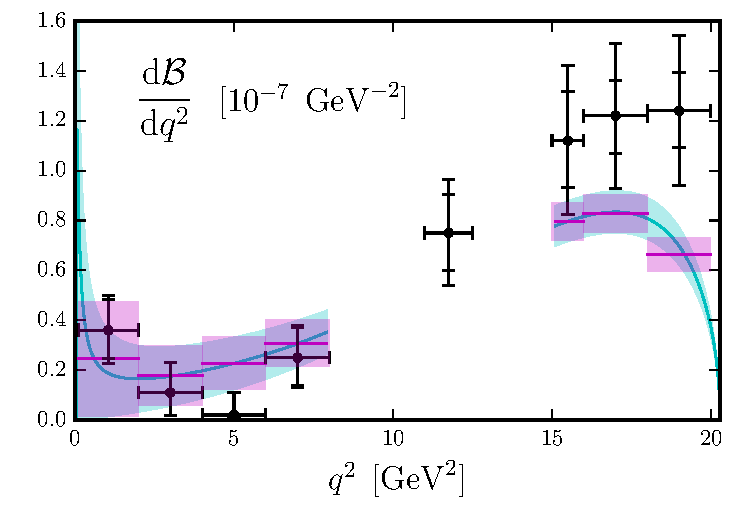
\includegraphics[width=0.6\textwidth]{Lmumu/figs/NewPredictions/fig8.pdf}
\caption{  Measurement of the differential branching fraction of the \decay{\Lb}{\Lz\mumu} decay
	as a function of \qsq already presented in Ch.~\ref{sec:Lmumu_intro} with improved Standard 
	Model predictions from Ref.~\cite{Detmold:2016pkz} overlaid.
 }
\end{figure}

  \begin{figure}[h!]
\centering
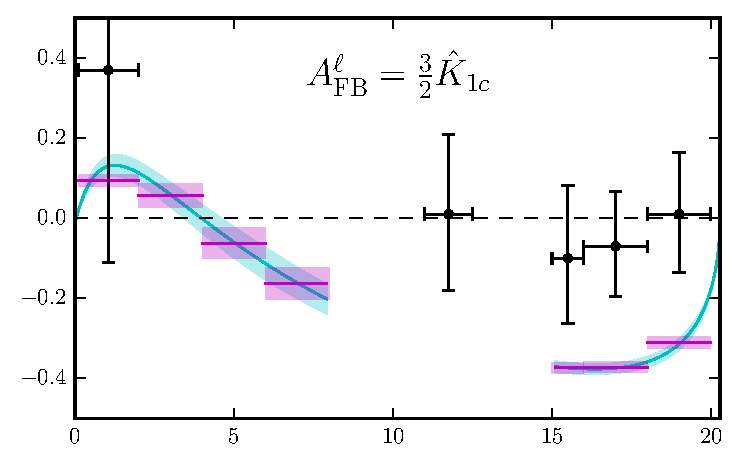
\includegraphics[width=0.6\textwidth]{Lmumu/figs/NewPredictions/fig9b.pdf}
\caption{  Measurement of the lepton side forward-backward asymmetry, \afbl, 
	as a function of \qsq already presented in Ch.~\ref{sec:ang_ana} with improved Standard 
	Model predictions from Ref.~\cite{Detmold:2016pkz} overlaid.
 }
\end{figure}

  \begin{figure}[h!]
\centering
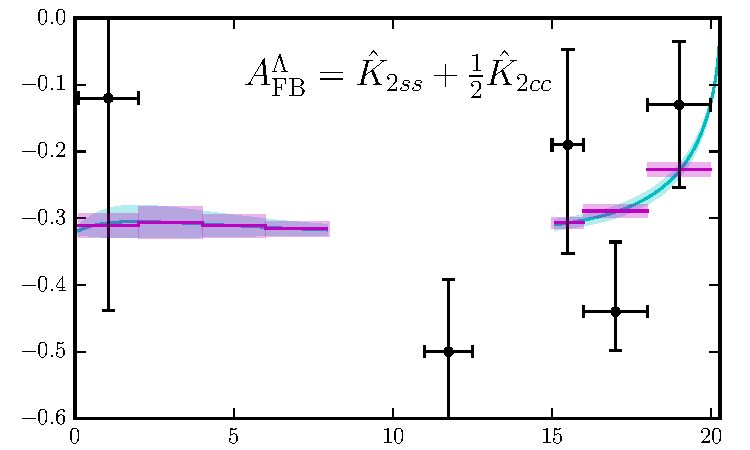
\includegraphics[width=0.6\textwidth]{Lmumu/figs/NewPredictions/fig9c.pdf}
\caption{  Measurement of the hadron side forward-backward asymmetry, \afbh, 
	as a function of \qsq already presented in Ch.~\ref{sec:ang_ana} with improved Standard 
	Model predictions from Ref.~\cite{Detmold:2016pkz} overlaid.
 }
\end{figure}

  \begin{figure}[h!]
\centering
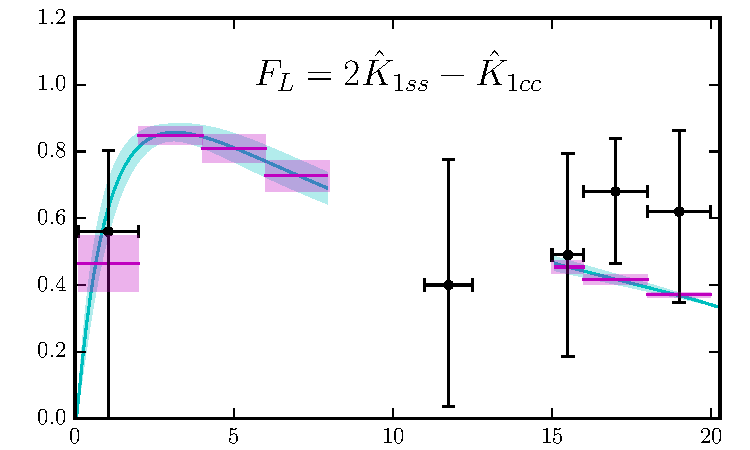
\includegraphics[width=0.6\textwidth]{Lmumu/figs/NewPredictions/fig9a.pdf}
\caption{  Measurement of the fraction of longitudinally polarised dimuons, \fl, 
	as a function of \qsq already presented in Ch.~\ref{sec:ang_ana} with improved Standard 
	Model predictions from Ref.~\cite{Detmold:2016pkz} overlaid.
 }
\end{figure}
  